\chapter{Modellierung}\label{cha:modellierung}

\section{Datenmodellierung}

Modellieren ist der Weg von der realen Welt bis zum Datenmodell. Ein Datenmodell verdeutlicht die Beziehungen zwischen Daten. Ergebnis des Modellierungsprozesses ist ein sogenanntes Datenschema, das zumeist grafisch visualisiert wird.
Im Hinblick auf die Datenmodellierung eignen sich folgende Ansätze:

\paragraph{Konzeptuelles Datenmodell}
Beschreibt die globale logische Struktur aller Daten Implementierungs-unabhängig und stellt diese in einer systematischen Form dar.

\begin{figure}[h]
    \centering
    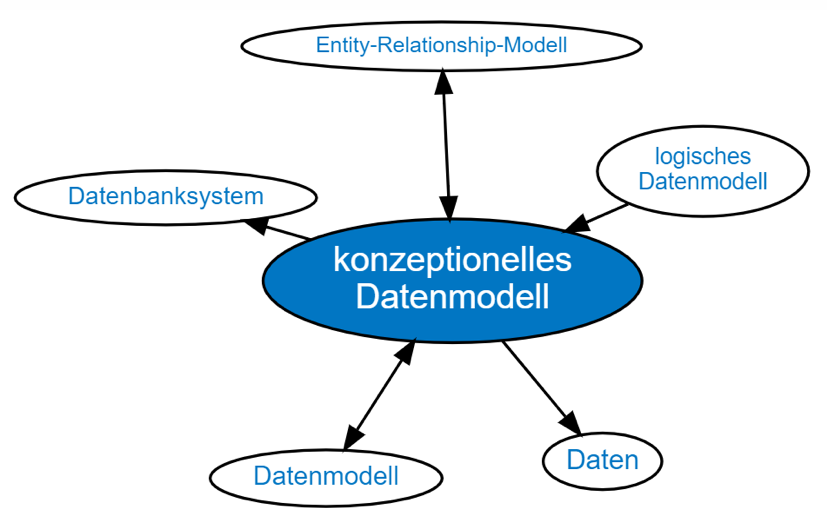
\includegraphics[width=.75\textwidth]{Content/images/modellierung/konzeptionell.png}
    \caption{Konzeptuelles Datenmodell}
    \label{fig:modellierung:konzeptuell}
 \end{figure}

 \paragraph{Logisches Datenmodell}
 Auf die spätere Implementierung ausgerichtetes Datenmodell, das die Daten für den späteren Einsatz bereits vorstrukturiert.

 \begin{figure}[h]
    \centering
    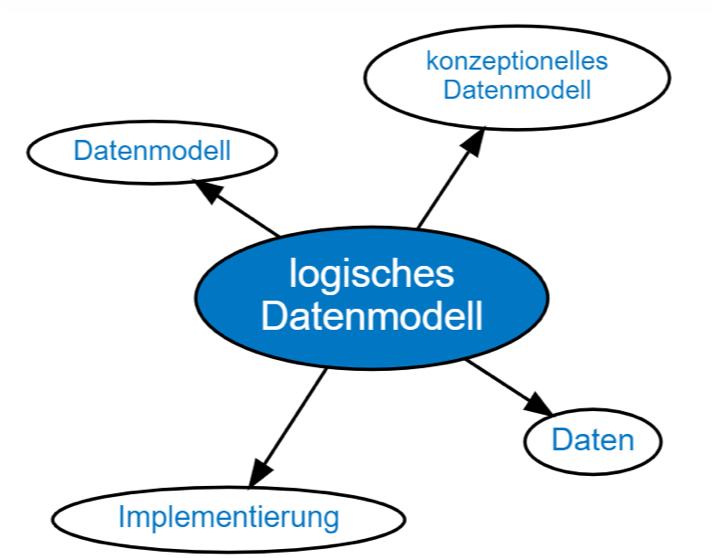
\includegraphics[width=.75\textwidth]{Content/images/modellierung/logisch.png}
    \caption{Logisches Datenmodell}
    \label{fig:modellierung:logisch}
 \end{figure}

 \paragraph{Physisches Datenmodell}
Basiert auf der Grundlage des logischen Datenmodells. Im physischen Datenmodell wird besonders auf Effizienz der SQL-Abfragen geachtet, beispielsweise durch den Entwurf von Indexstrukturen.

Aufgabe der Datenmodellierung ist es, bei der Konzeption eines Informationssystems dessen \emph{Objekte mittels Attribute und Beziehungen gemäß den Anforderungen zu strukturieren} und diese Struktur formal zu dokumentieren.

\emph{Ziele: Redundanzfreie Datenspeicherung und hohe Datenkonsistenz.}
Eine redundanzfreie Datenspeicherung liegt dann vor, wenn jede Information in einer Datenbank genau einmal vorkommt. Des Weiteren muss eine hohe Datenkonsistenz verfolgt werden, so dass Daten eindeutige Informationen darstellen.

\section{Datenmodelle}

Ein Modell ist ein \emph{vereinfachtes Abbild der Wirklichkeit.} Zur Beschreibung der Art und Weise, wie Daten in einer Datenbank gespeichert werden, gibt es verschiedene Datenmodelle. Einige dieser Modelle findet man auch in der betriebswirtschaftlichen Organisationslehre wieder.

\subsection{Hierarchisches Datenmodell}

Das hierarchische Datenmodell kennen wir vom Dateisystem unserer Festplatte (Laufwerksbuchstabe, Ordner, Dateien). Dieses Modell wird auch „Baumstruktur“ genannt. Ganz links (oder oben) befindet sich die Wurzel (Root). Von ihr sind alle Objekte abhängig, die weitere abhängige Objekte haben können. In der betriebswirtschaftlichen Lehre ist es mit einer Stablinienorganisation vergleichbar. Das hierarchische Datenmodell war früher ein sehr gebräuchliches Modell, deshalb bildet es die Grundlage älterer Datenbanksysteme.

\begin{figure}[h]
    \centering
    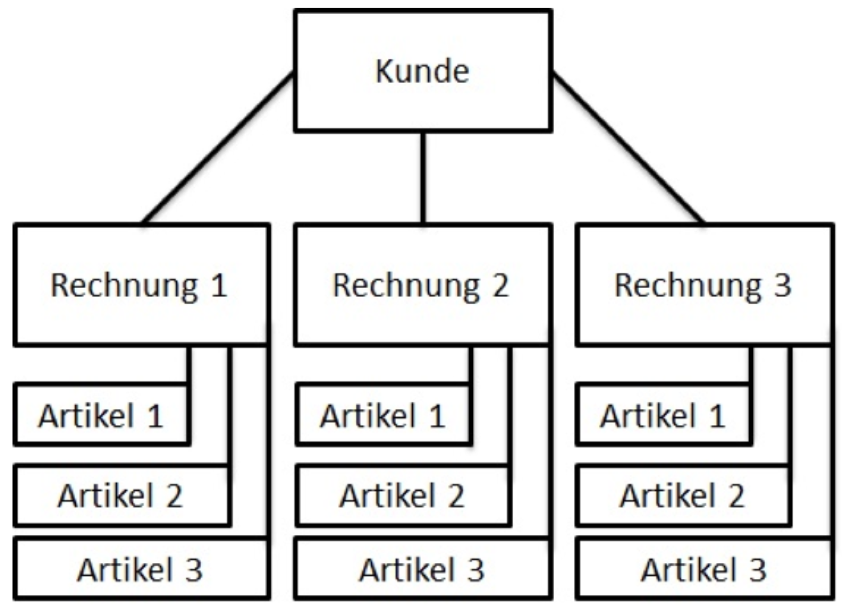
\includegraphics[width=.75\textwidth]{Content/images/modellierung/stablinien.png}
    \caption{Stablinienorganisation}
    \label{fig:modellierung:stablinien}
 \end{figure}

 Durch die \emph{hierarchische Baumstruktur ist der lesende Zugriff extrem schnell.} Der Nachteil der baumstrukturierten Verweise liegt bei der Speicherung der Daten und deren Verknüpfungen, da die Verweise untereinander vorab ermittelt werden müssen. Die Verknüpfungen werden über Eltern-Kind-Beziehungen realisiert und in der Baumstruktur abgebildet. Der große Nachteil bei diesem Modell ist es, dass man nur eine Baumstruktur verwenden kann: Es ist also nicht möglich, zwei Baumstrukturen miteinander zu verknüpfen. \emph{Das hat zur Folge, dass dieses Modell sehr starr ist und wenig Freiheit für den Entwickler bietet. }

 \subsection{Netzwerk Datenmodell}

Definition: Datenmodell, mit dem Netzwerkstrukturen zwischen Datensätzen beschrieben werden können.
Es dient als Grundlage vieler Datenbanksysteme. Die drei Datenbanksprachen DML, DDL und DCL werden angewandt. Durch das netzwerkartige Modell existieren meist unterschiedliche Suchwege, um einen bestimmten Datensatz zu ermitteln. Es ähnelt dem hierarchischen Datenbankmodell und kann einer Matrixorganisation gegenübergestellt werden. 
Das Netzwerk Datenbankmodell besitzt keine strenge Hierarchie. Ein Datenfeld besteht aus einem Namen und einem Wert.
Es sind m:n Beziehungen möglich, d.h. ein Datensatz kann mehrere Vorgänger haben. Des Weiteren können auch mehrere Datensätze an erster Stelle stehen. Der Vorteil dieses Modells ist, das es unterschiedliche Suchwege als Lösungsweg angibt, was natürlich auch zu Problemen führen kann, wenn der Entwickler genau einen Lösungsweg benutzen will. Auch die Übersichtlichkeit verringert sich, wenn das Modell ständig weiter wächst.

\begin{figure}[h]
    \centering
    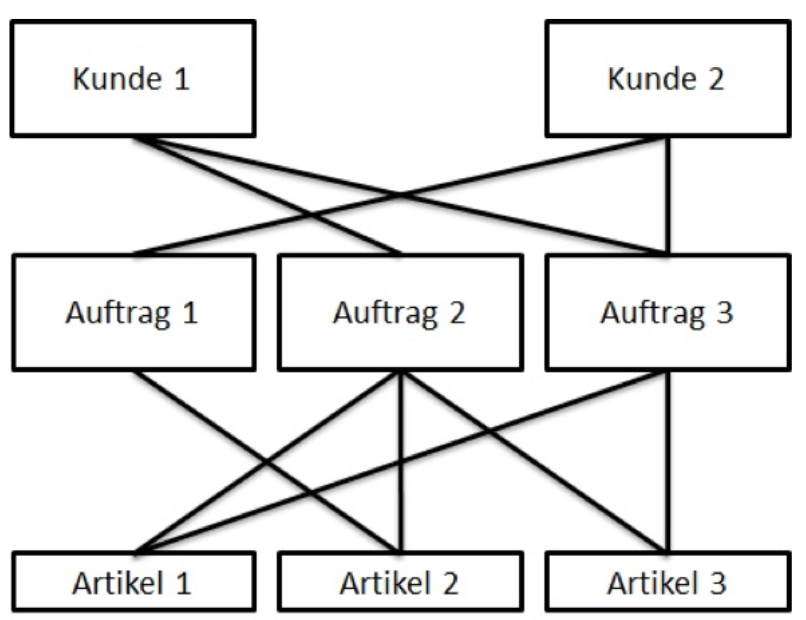
\includegraphics[width=.75\textwidth]{Content/images/modellierung/netzwerk.png}
    \caption{Netzwerk Datenmodell}
    \label{fig:modellierung:netzwerk}
 \end{figure}

 Heute wird das Netzwerkdatenbankmodell als eine Art Verallgemeinerung des hierarchischen Datenbankmodells gesehen.

 \subsection{Relationales Datenmodell}

 = Auf den Arbeiten von Edgar F. Codd von 1970 basierendes Datenmodell, mit dem Beziehungen zwischen Daten in Form von Relationen beschrieben werden. 

In einfachen Worten: Ein relationales Datenmodell ist eine Ansammlung von Tabellen, die miteinander verknüpft sind.
Das relationale Datenmodell ist das am weitesten verbreitete Datenmodell, welches in der Datenbankentwicklung als Standard genutzt wird. Das Fundament des Datenbankmodells besteht aus drei Elementen: Tabellen, Attributen und Beziehungen.

\paragraph{Vorteile:} sehr einfach und flexibel zu erstellen, hohe Flexibilität, leichte Handhabung
\paragraph{Nachteil:} Effizienzprobleme bei großem Datenvolumen

Die wichtigsten Operationen mit Relationen (relationale Algebra), die ein Datenbankmanagementsystem zur Verfügung stellen muss, sind folgende:

\begin{itemize}
    \item Auswahl von Zeilen
    \item Auswahl von Spalten
    \item Aneinanderfügen von Tabellen
    \item Verbund von Tabellen
\end{itemize}

\subsubsection{Entität}

Als Entität wird in der Datenmodellierung ein eindeutig zu bestimmendes Objekt bezeichnet, über das Informationen gespeichert oder verarbeitet werden sollen. Ein Entitätstyp beschreibt die Ausprägungen eines Objektes durch die Angabe von Attributen. Durch Typisierung (Erkennen gleicher Attribute von Entitäten) können Entitätstypen abgeleitet werden – aus mehreren Personen werden z.B. Kunden. Eine Entität kann materiell oder immateriell, konkret oder abstrakt sein. Beispiele für Entitäten: Fahrzeug, Konto, Person.

\subsubsection{Attribute in einer Entität}

Jede Entität besitzt eine bestimmbare Anzahl an Attributen (Ausprägungen bzw. Eigenschaften), die sich eindeutig von anderen Entitäten des gleichen Entitätstyps abgrenzen. Eine Eigenschaft ist ein konkreter Attributwert, den ein zuvor definiertes Attribut annehmen kann. Die Attribute stellen einen „Bauplan“ dar, der eine abstrakte Abbildung der Wirklichkeit ist.

\begin{figure}[h]
    \centering
    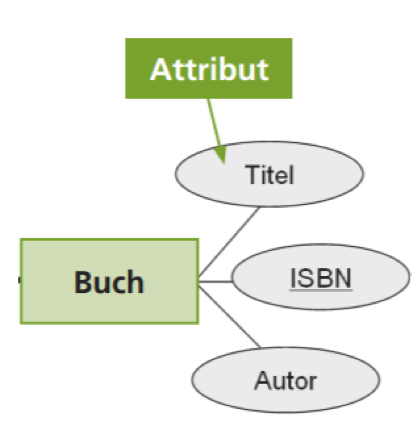
\includegraphics[width=.4\textwidth]{Content/images/modellierung/entity.png}
    \caption{Attribute einer Entity}
    \label{fig:modellierung:entity}
 \end{figure}

 Die Attribute in einer Entität können unterschiedlich aufgebaut sein. Man unterscheidet zwischen \emph{zusammengesetzte, mehrwertige und abgeleitete} Attribute.

 \paragraph{Zusammengesetzte Attribute} bestehen aus der Kombination mehrerer Attribute, die inhaltlich zusammengehören. Anhand einer Firmenadresse wird dies deutlich. Die Firmenadresse selbst ist ein Attribut der Firma, sie enthält aber die Attribute Straße, Hausnummer, Postleitzahl und Ort.

 \paragraph{Mehrwertige Attribute} können einen oder mehrere Attributwerte aufnehmen. So könnte ein Student gleichzeitig in zwei Studiengänge eingeschrieben sein.

 \paragraph{Abgeleitete Attribute} werden aus anderen Attributen oder Entitäten berechnet. Bezogen auf eine Datenbank wäre das z.B. die Bildung einer Summe aus mehreren Spalten einer Tabelle.
